\paragraph{ISO/IEC 9126}
Lo standard ISO/IEC 9126 si occupa di presentare le caratteristiche di qualità di un prodotto software e gli attributi che le compongono.

\begin{figure}[h]
    \centering
    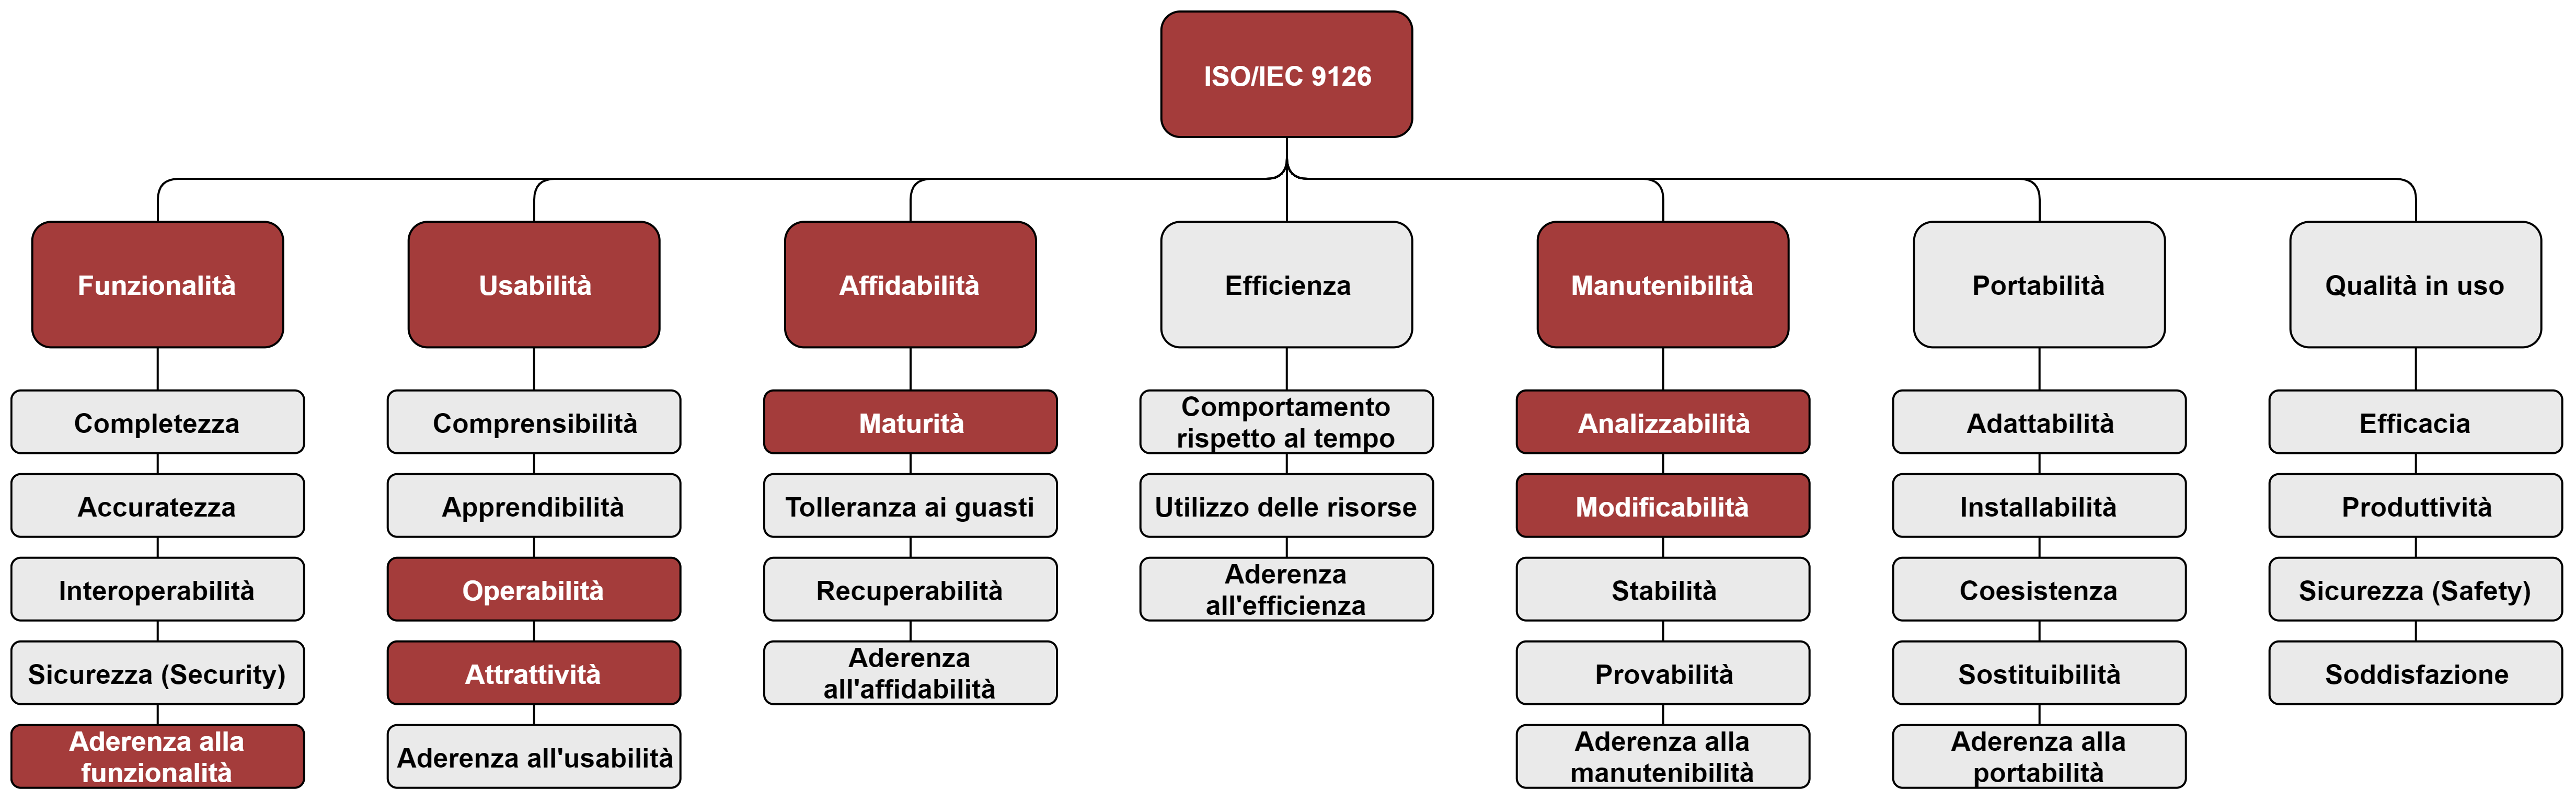
\includegraphics[scale=0.53]{Immagini/IsoIec9126.png}
    \caption{Schema dello standard ISO/IEC 9126. In rosso sono indicate le caratteristiche e attributi di interesse per il progetto.}
\end{figure}

\subparagraph{Metriche esterne}
Le metriche relative alla qualità "esterna" indirizzano le caratteristiche esteriori del software, cioè quelle rilevabili direttamente dagli utenti e dagli operatori.

\subparagraph{Metriche interne}
 Le metriche della qualità "interne" del software sono utilizzate durante la fase di sviluppo e permettono di valutare il comportamento del software dal punto di vista degli sviluppatori e di predire quello che sarà il punto di vista esterno degli utenti.

\subparagraph{Funzionalità}
Capacità del prodotto software di fornire funzioni adeguate al contesto di applicazione.
\begin{itemize}
\item \textbf{Adeguatezza}: Capacità di fornire un insieme di funzioni che permettano agli utenti del software di poter svolgere i loro compiti;
\item \textbf{Accuratezza}: Capacità di fornire i risultati attesi dall’utente con la precisione richiesta;
\item \textbf{Interoperabilità}: Capacità di interagire con uno o più sistemi specificati;
\item \textbf{Sicurezza (Security)}: Capacità di proteggere le informazioni e i dati dell’utente da persone non autorizzate ad accedervi;
\item \textbf{Aderenza alla funzionalità}: Capacità di aderire a standard, norme, convenzioni e regolamenti sulle funzionalità.
\end{itemize}

\subparagraph{Affidabilità}
Capacità del prodotto software di mantenere il livello di prestazione quando usato in condizioni specificate.
E’ limitata da errori nei requisiti, nella progettazione e nel codice del software.
\begin{itemize}
\item \textbf{Maturità}: Capacità di evitare che si verifichino errori.
\item \textbf{Tolleranza a guasti}: Capacità di mantenere il livello di prestazioni in caso di errori o violazione delle interfacce. Assieme alla \glo{Maturità}, descrivono l’attributo \glo{Disponibilità}, non specificato in quanto formato da questi due.
\item \textbf{Recuperabilità}: Capacità di ripristinare il livello di prestazioni e i dati in caso di errori e malfunzionamenti.
\item \textbf{Aderenza all’affidabilità}: Capacità di aderire a standard, norme, convenzioni e regolamenti sull’affidabilità.
\end{itemize}

\subparagraph{Usabilità}
Capacità del prodotto software di essere comprensibile, di poter essere studiato.
\begin{itemize}
\item \textbf{Comprensibilità}: Capacità di permettere all’utente di capire le funzionalità e come usarle con successo;
\item \textbf{Apprendibilità}: Capacità di permettere all’utente di imparare l’applicazione;
\item \textbf{Operabilità}: Capacità di permettere all’utente di usare il software e controllarlo;
\item \textbf{Attrattività}: Capacità di risultare attraente (ossia possedere una interfaccia utente accattivante);
\item \textbf{Aderenza all’usabilità}: Capacità di aderire a standard, norme, convenzioni e regolamenti sull’usabilità.
\end{itemize}

\subparagraph{Efficienza}
Capacità del prodotto software di realizzare le funzioni richieste nel minor tempo possibile.
\begin{itemize}
\item \textbf{Comportamento rispetto al tempo}: Capacità di fornire in tempi adeguati risposte per l’utente;
\item \textbf{Utilizzo risorse}: Capacità di utilizzare un appropriato numero e tipo di risorse, eseguendo le funzionalità previste;
\item \textbf{Aderenza all’efficienza}: Capacità di aderire a standard, norme, convenzioni e regolamenti sull’efficienza.
\end{itemize}

\subparagraph{Manutenibilità}
Capacità del prodotto software di essere modificato.
\begin{itemize}
\item \textbf{Analizzabilità}: Capacità di poter diagnosticare errori e individuare malfunzionamenti;
\item \textbf{Modificabilità}: Capacità di consentire lo sviluppo di modifiche al software originale;
\item \textbf{Stabilità}: Capacità di evitare effetti non desiderati;
\item \textbf{Provabilità}: Capacità di consentire la verifica delle funzionalità del prodotto software;
\item \textbf{Aderenza alla manutenibilità}: Capacità di aderire a standard, norme, convenzioni e regolamenti sulla manutenibilità.
\end{itemize}

\subparagraph{Portabilità}
Capacità di essere trasportato da un ambiente ad un altro.
\begin{itemize}
\item \textbf{Adattabilità}: Verrà descritta se ce ne sarà il bisogno;
\item \textbf{Installabilità}: Verrà descritta se ce ne sarà il bisogno;
\item \textbf{Coesistenza}: Verrà descritta se ce ne sarà il bisogno;
\item \textbf{Aderenza alla portabilità}: Verrà descritta se ce ne sarà il bisogno.
\end{itemize}

\subparagraph{Qualità in uso}
\begin{itemize}
\item \textbf{Efficacia}: Capacità per l’utente del prodotto software di raggiungere obiettivi specifici con \glo{accuratezza} e \glo{completezza};
\item \textbf{Produttività}: Capacità di permettere all’utente di impegnare un numero definito di risorse, in relazione all’efficienza raggiunta. Queste risorse possono essere tempo, materiali e costi;
\item \textbf{Sicurezza fisica (Safety)}: Capacità di raggiungere un livello accettabile di rischio per dati, business e persone. I rischi sono tipicamente correlati a difetti in progettazione o analisi o codifica;
\item \textbf{Soddisfazione}: Capacità di soddisfare gli utenti in uno specifico contesto.
\end{itemize}